\documentclass{article}
\usepackage[utf8]{inputenc}
\usepackage[english]{babel}
\usepackage{graphicx}
\usepackage{float}
\begin{document}
\title{A Better Front End for the Internet's Front Page: A Dream Interface for Reddit}
\author{Chris Dellomes\\
Professor: Dr. Dionisio\\
CMSI 370: Interaction Design\\
	Loyola Marymount University}

\date{November 24, 2015}

\maketitle

\begin{center}
\begin{abstract}
\noindent This study proposes an ideal user interface design utilizing the Reddit API. The design is meant to address the issue of navigation confusion by new users and enhance the presentation of information. Borrowing ideas from other popular websites, conforming to popular interface guidelines, and implementing voice based features, the design will provide the best possible experience for redditors.
\end{abstract}
\end{center}

\thispagestyle{empty}

\clearpage

\setcounter{page}{1}

\section{Introuction} When reddit.com launched back in June of 2005\cite{DMR}, it was a small social network site based on users submitting and voting on text posts and posted links. Over time, as Reddit implemented more features, such as giving users the ability to comment and create their own subredits, the number of redditors and subreddits grew exponentially\cite{Metrics}. As of October 2015, Reddit has 202 million unique visitors and over 800,000 subreddits, making reddit in the top 50 most popular web sites in the world\cite{Alexa, Reddit}. With the growing popularity of Reddit, the analysis of the site's current layout and the development of an improved user interface is a significant research topic.

\section{System Description} The design will utilize the Reddit API to allow users to post links and text submissions, make new subreddits, comment, and vote like the original site. However, the interface will present the content and allow users to interact with the content in a more natural and accessible manner. This investigation presents an ideal user interface design for the Reddit API that focuses on improving site navigation and adding voice functionality.

\begin{figure}[H]
\begin{center}
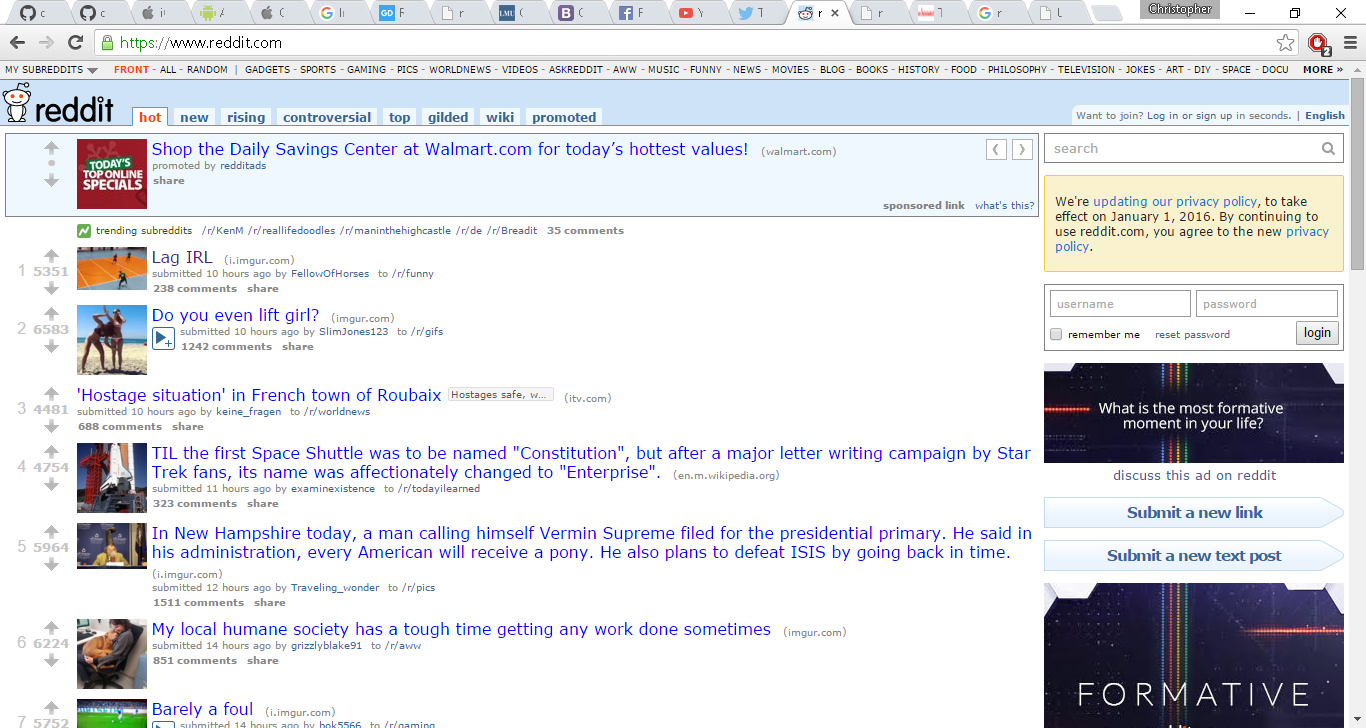
\includegraphics[width=1\textwidth]{reddit.png}
\caption{The current front page of reddit.}
\end{center}
\end{figure}

\indent The interface will implement voice recognition technology, similar to Siri for iOS or Cortana for Windows 10, in order for users to navigate and interact with content. On the original site, each post has an index, a net score of upvotes, comments with each one also having a net score of upvotes, and a subreddit which it was posted to. With voice recognition technology, navigating and interacting would be possible through voice commands, such as ``upvote post 1'', ``downvote comment by user Unidan'', ``go to the movies subreddit'', and ``post this text message...''. Integrating such technology into the reddit interface would allow users to control their reddit experience without requiring a mouse and keyboard. The implementation of voice recognition would be a powerful tool for users, especially physically impaired users who cannot interact with the content through external hardware.\\
\\
\indent While voice functionality is available, the proposed interface would still have an overall smooth sense of flow for users utilizing either a traditional mouse and keyboard setup or touch screen devices. The interface will coordinate with the Reddit API to ensure users remain capable of standard user abilities, like voting and posting. However, the interface will improve upon the current layout of Reddit's site by adopting aspects of other popular websites and popularly accepted interface guidelines, such as the OSX Human Guidelines and Google Material Design Principles.

\section{Top Level Design} While voice recognition is available, the proposed interface still accomodates keyboard and mouse or even touch sensitive devices by providing an elegant model. The main features of the interface are an overhead multipurpose navbar, fully interactive media objects, and toggle sidebar for navigating to subscribed subreddits.

\begin{figure}[H]
\begin{center}
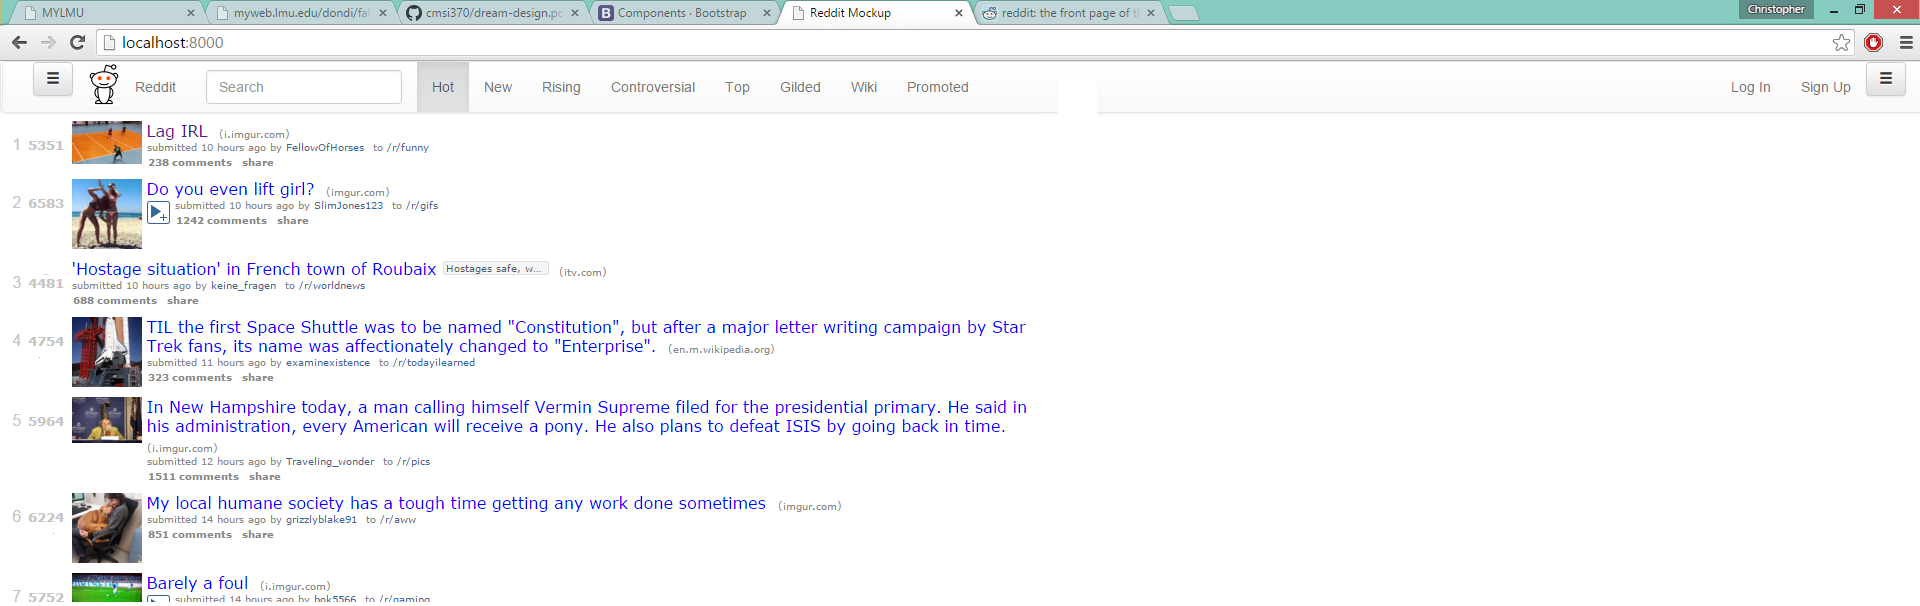
\includegraphics[width=1\textwidth]{mockup.png}
\caption{A mockup of the proposed interface design.}
\end{center}
\end{figure}

\subsection{Overhead Navbar} The design incorporates a constant overhead navbar at the top of the site with multiple related features. The navbar includes the search bar, a link to post a submission, as well as account related tabs, such as log in, sign up, and settings. The nav bar would also include the name of the current subreddit, the reddit logo, which would return the user to the site's front page when clicked, along with tabs for categories of posts, such as hot, new, rising, and top. Certain navbar tabs, like posting a submission and account settings would not be visible while the user is not logged in. Similarly, the sign up and login tabs would disappear while the user is currently logged into an account. For tabs which require another selection, such as when viewing top posts of all time, a smaller navbar would appear below the main one with tabs for filtering posts by submission date, such as past week, past month, and all time.

\begin{figure}[H]
\begin{center}
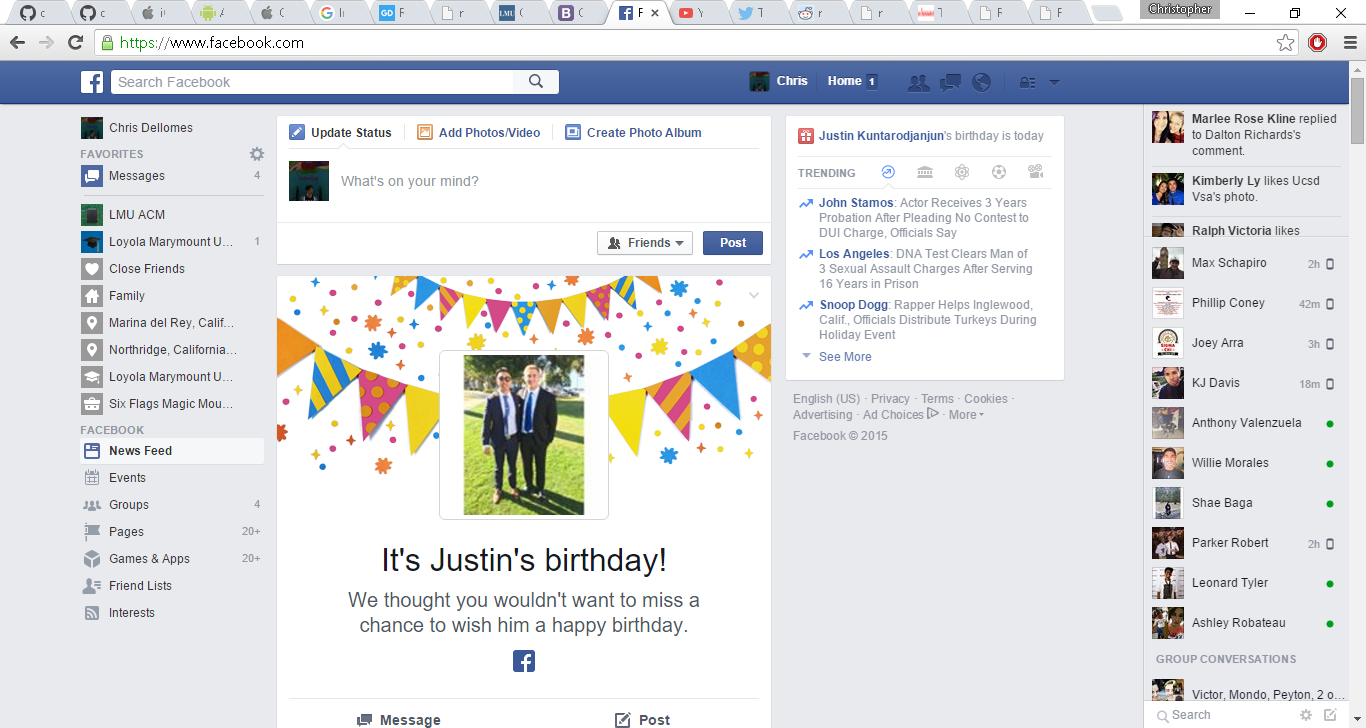
\includegraphics[width=1\textwidth]{navbar.png}
\caption{The navbar is similar to this one utilized by facebook in that it contains multiple functions, such as search and account settings, and remains at the top of the page even when scrolling.}
\end{center}
\end{figure}

\subsection{Interactive Media Objects} The interface maintains Reddit's traditional usage of media objects while expanding their overall interactivity. Like in the original site, media objects would include text which, when clicked, link the user to the text post and comments or linked article depending on the nature of the post. The media objects would also retain their quality of allowing the user to vote on the post, read the comments, share or save the post, and hide or report the post. The main difference in implementation would be that posts linked to pictures and gifs would produce a copy of the picture overlaying the window when either the text or the thumbnail is clicked. Similar to the post submission tab, the upvote and downvote buttons would be hidden until the user has met the required paramter of being logged into an account.

\begin{figure}[H]
\begin{center}
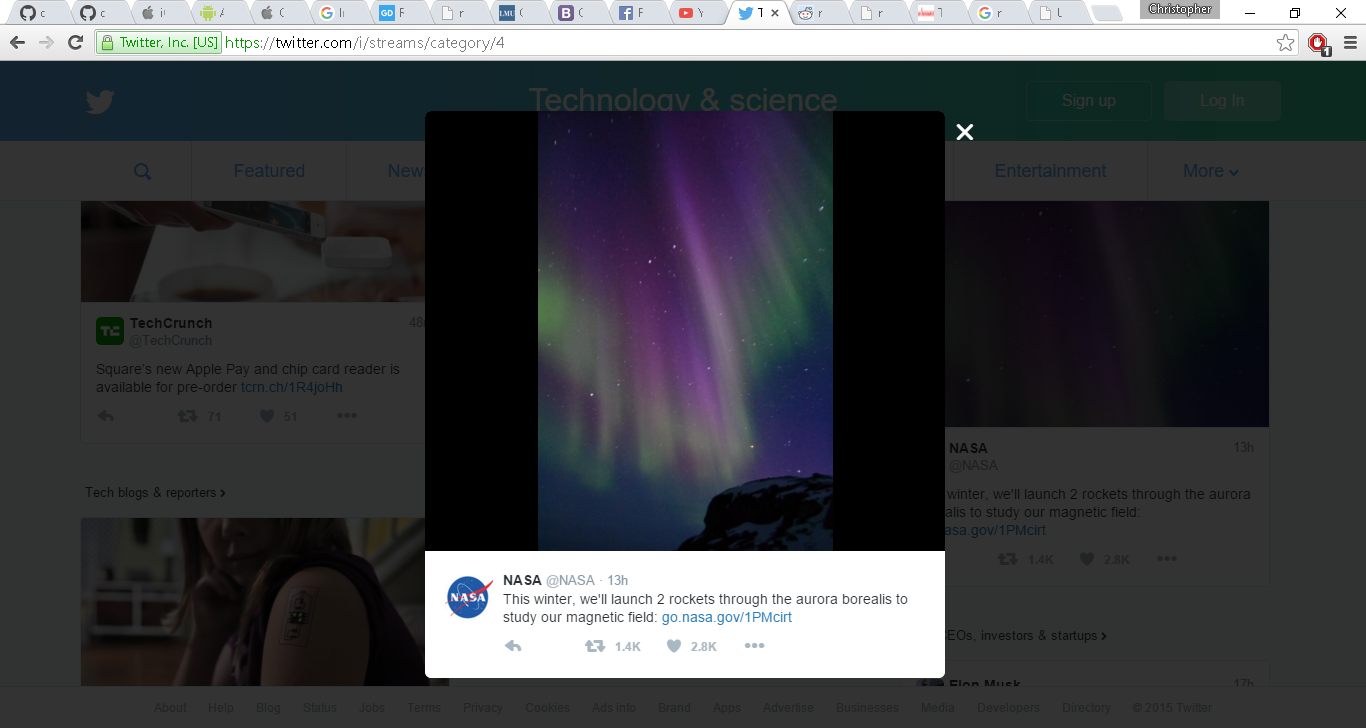
\includegraphics[width=1\textwidth]{media.png}
\caption{Similar to the above figure, when a post which features an image or gif is clicked, the content would appear in the center and overlay the screen, which is in the background and darkened for emphasis.}
\end{center}
\end{figure}

\subsection{Toggle Sidebars} The proposed interface design utilizes a sidebar that overlays the content on screen and can be toggled between being hidden and being shown. One of the sidebars will allow the user to subscribe to the current subreddit as well as include all of the user's subscribed subreddits which, when clicked, navigates the user to the selected subreddit. The other sidebar will display subreddit information, such as a subreddit description, moderators, and other relevant information. The sidebars will be able to be toggled by the click of a menu icon in the overhead navbar.

\begin{figure}[H]
\begin{center}
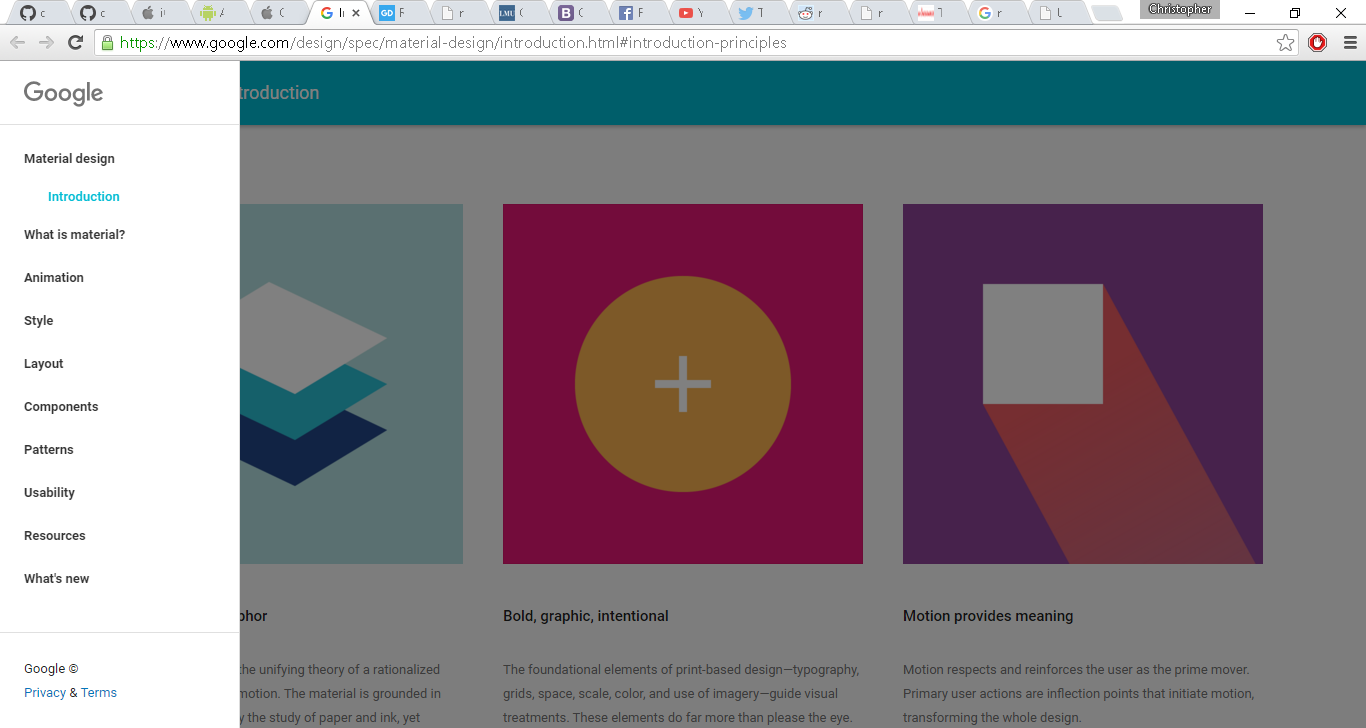
\includegraphics[width=1\textwidth]{sidebar.png}
\caption{The sidebar acts similar to the one in this figure by sliding in from the side overlaying the content on screen, which is in the background and darkened to provide emphasis, similar to the media objects.}
\end{center}
\end{figure}

\section{Usage Scenarios} Using the proposed user interface, there are multiple instances of usage scenarios. One such usage is when a redditor intends to post a submission. In the current site's format, the user is able to click on a button indicating the ability to post a submission to the site. However, the user is prompted with a login form instead of a content submission form in the case that the user has not yet logged into an existing account. The proposed interface design seeks to streamline the content submission process for users. If the user is not logged into an account, the submission post is hidden, keeping the function exclusive to logged in users. Once the user is logged in, however, the submission post tab becomes available and prompts the typical form for posting a submission. While Reddit's current system prompts a user to login when trying to post without an account, the proposed interface design hides those functions until the user is ready to acces them.\\
\\
\indent Another possible usage scenario for the proposed design is when a user tries to search for a specific subreddit. For the current site, the user enters a search term into a search bar near the top of the page. Closely related results are then presented to the user in the form of media objects, similar to posts. The proposed interface performs the task much in the same way. Except for placement of the search engine within the navbar, relevant posts and subreddits are presented in a similar manner. Since the current system follows the natural mental model for searching for things and is effective in the presentation of content, the ideal interface design maintains the overall performance of the search component.

\section{Rationale} The core rational behind the interface design choices is to properly align presentation and interaction with content with commonly accepted design principles to establish a familiar and recognizable landscape.

\subsection{Voice Controls} The purpose of including voice commands in the interface implementation would be to allow users to easily navigate the site without the need for external hardware. Voice commands allow users to directly translate thought into interaction with content without needing to physically move. Accomodating Don Norman's stages of action theory, use of a voice system would be more effective in bridging the gulf of execution between specifying the action and executing the action. There is less of a chance for errors if what the user wants to do can be directly relayed to the system to perform, as opposed to the user thinking of an action, navigating through the interface, and activating the appropriate component to perform the action.

\subsection{Overhead Navbar} The main purpose of the navbar is to keep the window uncluttered while maintaining functionality in a compact space. The navbar improves the overall experience by conforming to Apple's OSX and iOS Human Interface Guidelines for improving hierarchical navigation and reducing cluttering\cite{OSX, iOS}. The component also follows the Android Design Principles in that users are shown what actions they are capable of performing only once they have met the requirements\cite{Android}.

\subsection{Interactive Media Objects} The main purpose of this design choice is to preserve the current way in which content is projected by Reddit and maintain user familiarity with the site while at the same time removing the need for users to be redirected to a different website to view photos and gifs. This aspect of the interface design is meant to align with Google's Material Design principles in that the media objects no longer remove the user from the Reddit experience when interacted with\cite{Google}. By presenting images in such a way that overlays the site, the component also conforms to Apple's OSX Human Interface Guidelines in that the active image is highlighted and stands out from the rest of the content on screen\cite{OSX}.

\subsection{Toggle Sidebar} The core concept of this interface implementation is similar to the navbar in removing clutter from the window while compacting and maintaining general functionality. By keeping the sidebar hidden, but accessible from the navbar, the subreddit links do not interfere with current navigation while being easily accessible, facilitating a smooth transition from one subreddit to another. The intention of the component is to conform to Android Developer Principles by allowing users to access their saved data at any point while navigating the interface and displaying content only when users desire it.\cite{Android}.

\section{Usability Forecast} Although the proposed interface design has not been tested, we can analyze the overall design and construct a usability forecast.

\subsection{Learnability} If the proposed interface were implemented, I predict that the learnability of interface would perform just as well if not better than the original site format. In terms of presentation of content, the proposed interface preserves the original use of media objects to represent posts, maintaining the original site's learnability in interacting of posts. The overhead navbar centralizes many of the primary site functions, allowing for users to quickly find the function they intend to use. For an individual new to the interface and Reddit in general, they would not be able to learn how to post or vote on content until they loig in, which is not a signficant learnability issue considering those functions are not accessible without being logged in anyway. Additionally, the sidebars will be accessible through a menu icon, which will clearly indicate to users the existence of the additional menus, though users must explore the sidebars before learning what content they contain. Overall, the interface conforms to popularly accepted design principles, which creates a format users of similar social network sites are familiar with, thus improving general learnability.

\subsection{Efficiency} Efficiency is another strong point with the interface design. With the navbar remaining at the top of the screen at all times, users can easily switch between browsing content and performing site functions, like posting and searching. Also, with the navbar remaining present at all times, both sidebars are also accessible at any point, allowing for users to seamlessly and quickly navigate to other subscribed subreddits. This design choice improves upon the site's original layout, which requires users to renavigate to the top of the page in order to access the site functions. Also, by removing the need for users to navigate to a different webpage when viewing images or gifs, users can quickly transition back to content browsing without losing their place. The site's inclusion of voice recognition software also provides an effective means of performing an action and navigating without the need to physically navigate with a cursor or physically tap the button in the case of a mobile device.

\subsection{Error Rate} A potential source for errors is with the distinction between sidebars. This stems from the fact that the sidebars would use similar icons for access, causing users to potentially open one with the intention of accessing information found in the other. Though users may eventually recognize which sidebar contains what information, the potential for committed errors exists until that moment. Another potential source for errors would be users intending to post submission or vote on content without first being logged into an account. Since those features are hidden and unavailable until the user is logged in, a user familiar new to the site but familiar with the function could potentially spend a significant amount of time and make errors while trying to find the functions.

\subsection{Memorability} One memorability issue of the site would involve the distinction between the sidebars. Since the sidebars would use similar icons for access, it would be up to the user to remember which sidebar contained what content. There is the chance that a user could open a menu meaning to navigate to a subscribed subreddit, but accidently open the sidebar which contains the subreddit information. Though the subreddit information sidebar would be located on the right side of the screen, which would be what experienced redditors are familiar seeing on the original site format, newer users would potentially have trouble making the distinction. Besides the sidebar distinction, though, the overall layout of the designed interface and mental model fit closely with the site's original format and are therefore memorable to experienced users.

\subsection{Satisfaction} Users will be able to perform functions, transition between subreddits, and experience content effectively. Reddit's original use of content voting is an effective form of direct manipulation preserved by the introduced interface. Since it has been recorded that users respond positively to well executed direct manipulation, users should feel satisfied when browsing and interacting with content. The use of menus and forms, such as with filters and content submission, results in more complex tasks being divided into smaller portions, keeping the user from being overwhelmed. The overall satisfaction of the designed interface would be somewhat more signficant than Reddit's original site format.

\clearpage

\begin{thebibliography}{100}

\bibitem{Alexa} ``Alexa Top 500 Global Sites", \emph{Alexa Internet}, http://www.alexa.com/topsites
\bibitem{Android} ``Android Design Principles", \emph{Google Inc}, http://developer.android.com/design/get-started/principles.html
\bibitem{Google} ``Google Material Design", \emph{Google Inc}, https://www.google.com/design/spec/material-design/
\bibitem{Metrics} ``Reddit Metrics", \emph{Reddit Metrics} http://redditmetrics.com/history
\bibitem{Norman} Norman, Don, \emph{The Design of Everyday Things}. Basic Books Inc., New York, 1988
\bibitem{iOS} ``iOS Human Interface Guidelines", \emph{Apple Inc}, https://developer.apple.com
\bibitem{OSX} ``OS X Human Interface Guidelines", \emph{Apple Inc}, https://developer.apple.com
\bibitem{Reddit} ``Reddit About Page", \emph{Reddit Inc}, https://www.reddit.com/about/
\bibitem{DMR} ``Reddit Statistics", \emph{DMR}, http://expandedramblings.com/index.php/reddit-stats/

\end{thebibliography}

\end{document}